%%%%%%%%%%%%%%%%%%%%%%%%%%%%%%%%%%%%%%%%%
% Beamer Presentation
% LaTeX Template
% Version 1.0 (10/11/12)
%
% This template has been downloaded from:
% http://www.LaTeXTemplates.com
%
% License:
% CC BY-NC-SA 3.0 (http://creativecommons.org/licenses/by-nc-sa/3.0/)
%
%%%%%%%%%%%%%%%%%%%%%%%%%%%%%%%%%%%%%%%%%

%----------------------------------------------------------------------------------------
%	PACKAGES AND THEMES
%----------------------------------------------------------------------------------------

\documentclass{beamer}

\mode<presentation> {

% The Beamer class comes with a number of default slide themes
% which change the colors and layouts of slides. Below this is a list
% of all the themes, uncomment each in turn to see what they look like.

%\usetheme{default}
%\usetheme{AnnArbor}
%\usetheme{Antibes}
%\usetheme{Bergen}
%\usetheme{Berkeley}
%\usetheme{Berlin}
%\usetheme{Boadilla}
%\usetheme{CambridgeUS}
%\usetheme{Copenhagen}
%\usetheme{Darmstadt}
%\usetheme{Dresden}
%\usetheme{Frankfurt}
%\usetheme{Goettingen}
%\usetheme{Hannover}
%\usetheme{Ilmenau}
%\usetheme{JuanLesPins}
%\usetheme{Luebeck}
%\usetheme{Madrid}
%\usetheme{Malmoe}
%\usetheme{Marburg}
\usetheme{Montpellier}
%\usetheme{PaloAlto}
%\usetheme{Pittsburgh}
%\usetheme{Rochester}
%\usetheme{Singapore}
%\usetheme{Szeged}
%\usetheme{Warsaw}

% As well as themes, the Beamer class has a number of color themes
% for any slide theme. Uncomment each of these in turn to see how it
% changes the colors of your current slide theme.

%\usecolortheme{albatross}
%\usecolortheme{beaver}
%\usecolortheme{beetle}
%\usecolortheme{crane}
%\usecolortheme{dolphin}
%\usecolortheme{dove}
%\usecolortheme{fly}
%\usecolortheme{lily}
%\usecolortheme{orchid}
%\usecolortheme{rose}
%\usecolortheme{seagull}
%\usecolortheme{seahorse}
%\usecolortheme{whale}
%\usecolortheme{wolverine}

%\setbeamertemplate{footline} % To remove the footer line in all slides uncomment this line
%\setbeamertemplate{footline}[page number] % To replace the footer line in all slides with a simple slide count uncomment this line

%\setbeamertemplate{navigation symbols}{} % To remove the navigation symbols from the bottom of all slides uncomment this line
}

\usepackage{graphicx} % Allows including images
\usepackage{booktabs} % Allows the use of \toprule, \midrule and \bottomrule in tables

%----------------------------------------------------------------------------------------
%	TITLE PAGE
%----------------------------------------------------------------------------------------

\title[Mastering Metrics]{Understanding Metrics based on Mastering Metrics } % The short title appears at the bottom of every slide, the full title is only on the title page

\author{Corinna Birner \& Max M{\"u}ller} % Your name
\institute[JMU] % Your institution as it will appear on the bottom of every slide, may be shorthand to save space
{University of W{\"u}rzburg }\\ % Your institution for the title page
\medskip
\textit{{corinna.birner@stud-mail.uni-wuerzburg.de 
max.mueller@stud-mail.uni-wuerzburg.de} % Your email address
}
\date{\today} % Date, can be changed to a custom date

%------------------------------------------------
\begin{document}

\begin{frame}
\titlepage % Print the title page as the first slide
\end{frame}

%------------------------------------------------
\begin{frame}
\begin{center}
\textbf\Huge{Chapter 3: Instrumental Variables}
\end{center}
\end{frame}

%------------------------------------------------
\begin{frame}
\frametitle{Overview} % Table of contents slide, comment this block out to remove it
	\begin{itemize}
		\item today we will continue our journey on the path from cause to effect 
		\item we just learned that regression is a powerful tool for estimation
		\item sometimes the forces of nature, especially human nature, can manipulate our treatment in a way that can help us find causal effects using the instrumental variable (IV) method 
		\item we will therefore look at three case studies today:
\end{itemize}
\tableofcontents % Throughout your presentation, if you choose to use \section{} and \subsection{} commands, these will automatically be printed on this slide as an overview of your presentation
\end{frame}

%----------------------------------------------------------------------------------------
%	PRESENTATION SLIDES
%----------------------------------------------------------------------------------------

%------------------------------------------------

%------------------------------------------------
%------------------------------------------------
\section{Charter vs. Public Schools: KIPP Lynn} % Sections can be created in order to organize your presentation into discrete blocks, all sections and subsections are automatically printed in the table of contents as an overview of the talk

%------------------------------------------------

%\subsection{Even more Nonsense} % A subsection can be created just before a set of slides with a common theme to further break down your presentation into chunks


%------------------------------------------------
\begin{frame}
\frametitle{Charter Schools in the USA}
	\begin{itemize}
		\item public schools in the USA often have a bad reputation
		\item charter schools are public schools but operated by a NGO
		\item charter schools have more autonomy and can structure their curricula more independently
		\item a NGO gets a charter for a limited period and the renewal depends on good performance
		
	\end{itemize}


\end{frame}

%------------------------------------------------
\begin{frame}
\frametitle{do charter schools provide better public education?}
\begin{itemize}
\item one approach to education is the No Excuses approach which uses long school days and selective teacher hiring and focuses on discipline and math and reading skills
		\item one emplemantic example of this approach is the Knowledge Is Power Program (KIPP)
		\item this program recruits teachers from the best colleges to teach in low-performing school districts
		\item KIPP's students: 95 \% black and hispanic, 80 \% poor
		\item nonwhite KIPP students have higher test scores than nonwhite students from nearby schools \\~\\
		
		\item Is there a causal effect of the KIPP System?
	\end{itemize}
\end{frame}

%------------------------------------------------
\begin{frame}
\frametitle{Case Study: KIPP Lynn}
\begin{itemize}
\item in order to answer this question we will look at KIPP at the city of Lynn in Massachusetts
\item KIPP Lynn opened in 2004 and after one year over 200 students applied for only 90 seats
\item Massachusetts law requires scarce charter seats to be allocated by lottery
\item the decission to go to the charter school is never entirely random 
\item however, we can still compare applicants who are and who are not offered a seat as a result of the random admission lottery
\item we can use the IV tool on the lottery in order to frame a naturally occuring randomized trial
\end{itemize}

\end{frame}
%------------------------------------------------
\begin{frame}
\frametitle{Case Study: KIPP Lynn}
\begin{itemize}
\item IV turns randomized offer effects into causal estimates of the efffect of charter attendance
\item IV captures effects on the sort of child who enrolls in KIPP when offered a seat but wouldn't get in otherwise
\item this group is called compliers 
\item KIPP Study details:
	\begin{itemize}
		\item lotteries from 2005 to 2008
		\item 446 applicants
		\item some applicnts were excluded (too old) or bypass the lottery (enrolled sibling)
		\item outcome: standardized math/verbal score
	\end{itemize}
\end{itemize}

\end{frame}


%------------------------------------------------
\begin{frame}
\frametitle{Application and enrollment process for KIPP Lynn}

\begin{columns}
\column{.5\textwidth}
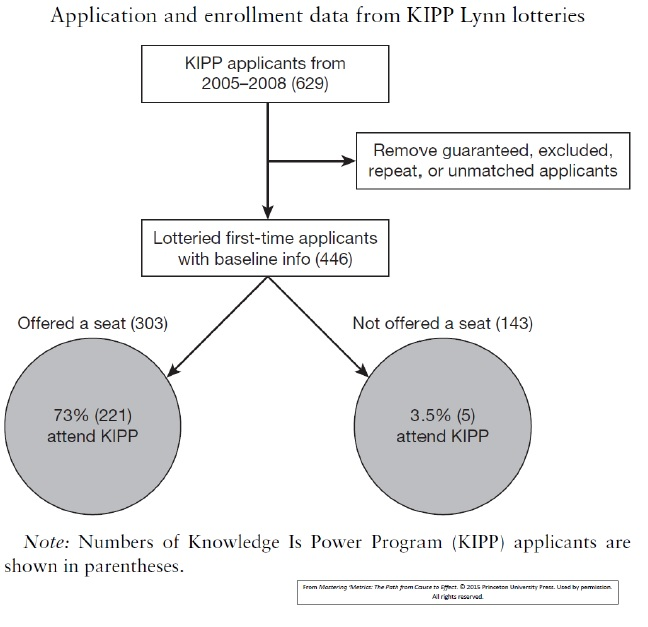
\includegraphics[width=6.5cm,height=6.5cm,keepaspectratio]{Figure 3.1} 

\column{.45\textwidth}
\begin{itemize}
	\item removed because of age, enrolled siblings, etc.
	\item only 73\% attended KIPP, the others moved away or decided to attend a different school
	\item 3,5 \% were offered a seat afterwards although they had lost in the lottery
\end{itemize}

\end{columns}
\end{frame}

%------------------------------------------------
\begin{frame}
\frametitle{KIPP Lynn Baseline Characteristics}

\begin{columns}
\column{.5\textwidth}
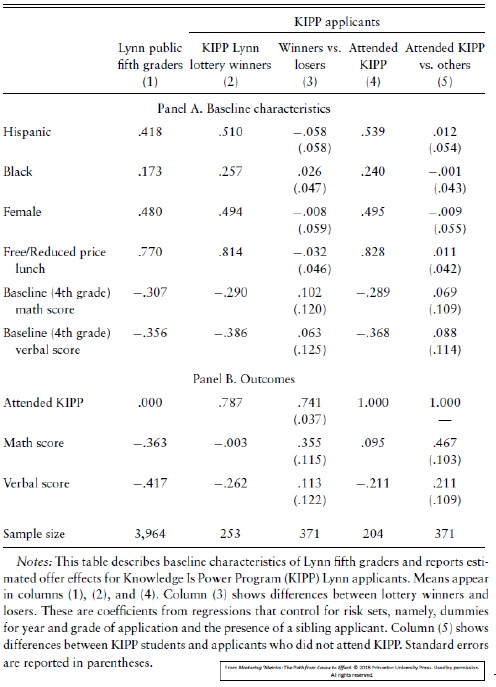
\includegraphics[width=6.5cm,height=6.5cm,keepaspectratio]{Table 3.1} 

\column{.45\textwidth}
\begin{itemize}
	\item only small differences between winners and losers in gender, ethnicity, economic status
	\item baseline scores $-.3\sigma$ below state mean
	\item insignificant pre-treatment differences between winners and losers (column 3)
\end{itemize}



\end{columns}
\end{frame}

%------------------------------------------------
\begin{frame}
\frametitle{KIPP Lynn Baseline Characteristics}

\begin{columns}
\column{.5\textwidth}
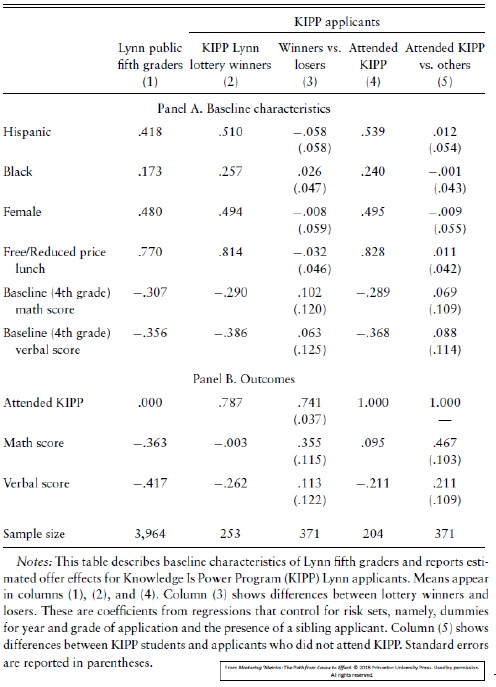
\includegraphics[width=6.5cm,height=6.5cm,keepaspectratio]{Table 3.1} 

\column{.45\textwidth}
\begin{itemize}
	\item there might be a selection bias for students enrolled and nonenrolled
	\item lottery winners who chose to go elsewhere might care less about school 
	\item no significant differences in column 5 
	\item selection bias might not be important in this context
\end{itemize}



\end{columns}
\end{frame}


%------------------------------------------------
\begin{frame}
\frametitle{KIPP Lynn - Outcomes}
\begin{columns}
\column{.5\textwidth}
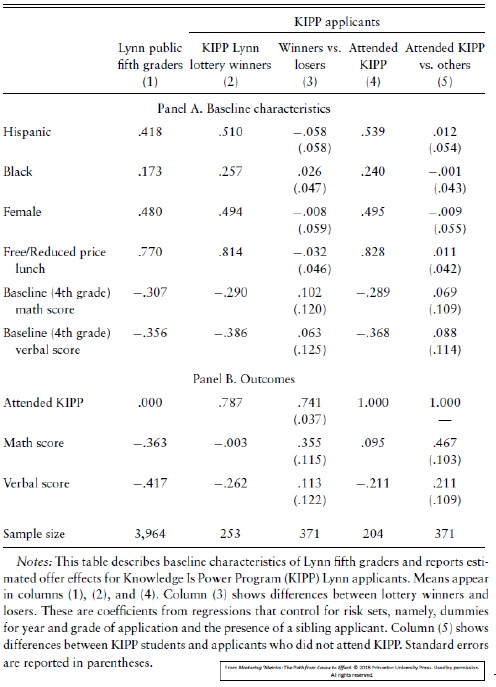
\includegraphics[width=6.5cm,height=6.5cm,keepaspectratio]{Table 3.1} 

\column{.45\textwidth}
\begin{itemize}
	\item math score of applicants who where offered a seat (post-treatment) is 0
	\item math score of average 5th grader is -.36
	\item average causal effect: the offer of a seat at KIPP boosts math score by $.36\sigma$
\end{itemize}

\end{columns}

\end{frame}

%%------------------------------------------------
\begin{frame}
\frametitle{Technical note on results in differences}
	\begin{itemize}
	\item results in column 3 are not differences in average 
	\item they come from a regression of scores on a dummy for KIPP offer, year, grade of application and presence of a sibbling
	\item this is needed because the probability of winning varies from year to year, between applicants from 5th and 6th grade and children with siblings
	\end{itemize}
\end{frame}

%%------------------------------------------------
\begin{frame}
\frametitle{KIPP Lynn Outcomes}
	\begin{itemize}
	\item what does the offer effect of $.36\sigma$ tell us about the effect of KIPP attendance?
	\item we need to turn the offer effect into an attendance effect by using the IV
	\item the instrumental variable here is a dummy indicating KIPP applicants who receive an offer
	\item our instrument must meet three requirements:
	\end{itemize}
\end{frame}

%------------------------------------------------
\begin{frame}
\frametitle{Instrumental Variables}
\begin{itemize}
\item first stage: the instrument has a causal effect on the variable whose effects we're trying to capture
\item independence assumption: the instrument is unrelated to the omitted variables
\item exclusion restriction: the instrument affects outcomes through a single channel
\end{itemize}


\end{frame}
%------------------------------------------------
\begin{frame}
\frametitle{The IV estimator in the KIPP Lynn}
Using these three assumptions, the IV method gets us a chain reaction leading from the instrument to student achievement
\begin{itemize}
\item first link connects randomily assigned offers with KIPP attendance 
\item second link connects KIPP attendance with achievement
\item with the independence assumption and the exclusion restriction the product of these two links generates the effect of offer on test scores:
\end{itemize}
$$Effect~of~offers~on~scores = $$
$$(Effect~of~scores~on~attendance ~x~Effect~of~attendance ~on ~scores)$$ \\~\\

The effect of KIPP attendance is: $$~Effect ~of ~attendance ~on ~scores = ~\frac{~Effect ~of ~offers ~on ~scores}{~Effect ~of ~offers ~on ~attendance}$$

\end{frame}

%------------------------------------------------
\begin{frame}
\frametitle{The IV estimator in the KIPP Lynn}
\begin{itemize}
\item KIPP offers are assumed to affect test scores via KIPP attendance alone
\item Offers increase attendance rates by .74\%
\item to get the attendance effect we multiply the effect of the ofers in scores by $\frac{1}{.74}$
\item raw difference is $.355\sigma$, so the effect turns out to be $.48\sigma$
\end{itemize}
\end{frame}

%------------------------------------------------
\begin{frame}
\frametitle{KIPP Lynn - Outcomes}
\begin{columns}
\column{.5\textwidth}
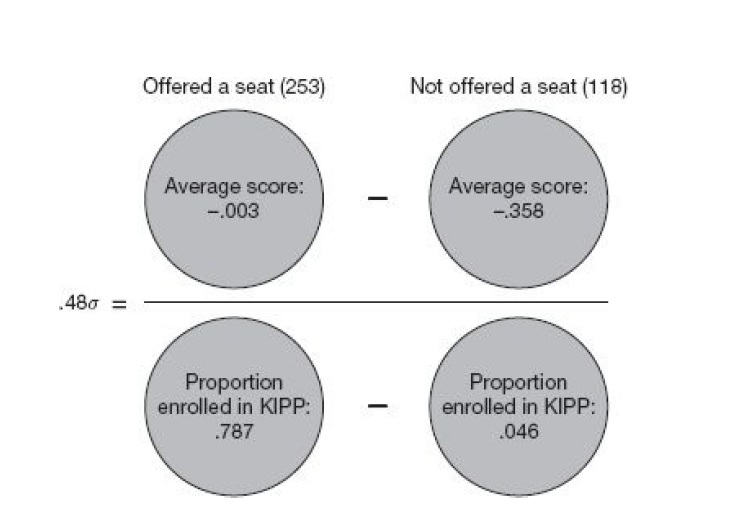
\includegraphics[width=6.5cm,height=6.5cm,keepaspectratio]{Figure 3.2} 

\column{.45\textwidth}
\begin{itemize}
	\item difference in math scores is $.355\sigma$
	\item offers in attendance is .741
	\item the effect of the KIPP enrollment is $.48\sigma$
\end{itemize}

\end{columns}

\end{frame}

%------------------------------------------------
\begin{frame}
\frametitle{The IV estimator}
Our IV estimation needs three ingredients:
\begin{itemize}
	\item the instrument $Z_i$: randomizes the treatment, here Dummy that indicates if KIPP seat was offered
	\item the treatment variable $D_i$ (sometimes called endogenous variable), here Dummy that indicates KIPP attendance
	\item the outcome variable $Y_i$: here the 5th grade math score
\end{itemize}



\end{frame}

%------------------------------------------------
\begin{frame}
\frametitle{The IV estimator}
Our IV chain reaction has multiple components:
\begin{itemize}
	\item the randomizer that is called instrument $Z_i$ (here: KIPP offer)
	\item first stage: effect of $Z_i$ on $D_i$: link from the instrument to the causal variable of interest (here: effect of offer on KIPP attendance)
	\item the direct effect of the instrument on outcomes $Z_i$ on $Y_i$ is called reduced form (here: effect of offers on scores)
	\item the causal effect of interest $D_i$ on $Y_i$ is determined by the ratio of reduced form to first-stage estimates and is called local average treatment effect (LATE)
\end{itemize}



\end{frame}

%------------------------------------------------
\begin{frame}
\frametitle{Estimating the LATE}
the first stage:
$$E[D_i|Z_i=1]-E[D_i|Z_i=0]~,~we ~call ~this ~\phi$$

difference in KIPP attendance between those offered and not offered a seat

the reduced form:
$$E[Y_i|Z_i=1]-E[Y_i|Z_i=0]~,~we ~call ~this ~\rho$$

difference in average scores between those offered and not offered a seat

the LATE:
$$\lambda = \frac{\rho}{\phi} = \frac{E[Y_i|Z_i=1]-E[Y_i|Z_i=0]}{E[D_i|Z_i=1]-E[D_i|Z_i=0]} $$
difference in scores between winners and losers divided by difference in attendance between winners and losers

\end{frame}


%------------------------------------------------
\begin{frame}
\frametitle{LATE in the KIPP Lynn}
\begin{itemize}
\item the LATE is the average causal effect or children whose enrollment status (KIPP vs. public) is determined solely by the KIPP lottery
\item we can think of four types of children in this scenario
	\begin{itemize}
		\item those who don't go to KIPP, even if they win a seat: never-takers
		\item those who go to KIPP, even if they lose in the lottery: always-taker
		\item those who go to KIPP if they win and don't go if they lose: compliers
		\item those who to KIPP only if they lose: defiers
	\end{itemize}
	\item the compliers are important for the IV because their treatment status is determined by the instrument
	\item we indicate this group with the dummy $C_i$
\end{itemize}

\end{frame}

%------------------------------------------------
\begin{frame}
\frametitle{What does LATE tell us?}

\begin{columns}
\column{.5\textwidth}
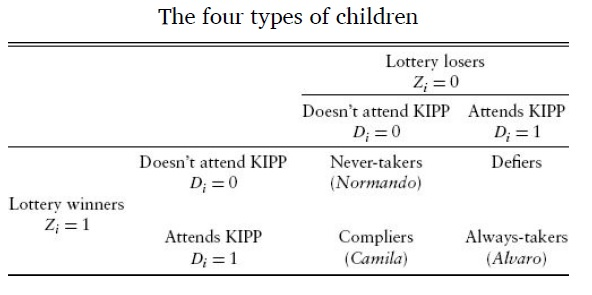
\includegraphics[width=6.5cm,height=6.5cm,keepaspectratio]{Table 3.2} 

\column{.45\textwidth}
\begin{itemize}
	\item four types of children: never-takers, always-takers, defiers, compliers
	\item LATE theorem says that the ratio of reduced form to first stage os LATE, the average causal effect of treatment on compliers
\end{itemize}

\end{columns}
\end{frame}


%------------------------------------------------
\begin{frame}
\frametitle{The LATE}
\begin{itemize}
\item LATE doesn't necesarrily describe causal effect for never-takers and always-takers
\item if you want to look at average causal effects for the entire treated population, you need to look at the treatment effect on the treated (TOT): $E[Y_1_i - Y_0_i|D_i =1]$ 
\item TOT includes always-takers and compliers
\item LATE and TOT are usually not the same
\item you should always think about the external validity of a particulat LATE
\end{itemize}
\end{frame}




%------------------------------------------------
\section{Police response to domestic violence: MDVE} 

\begin{frame}
\frametitle{The Minneapolis Domestic Violence Experiment (MDVE)}
\begin{itemize}
\item this experiment tried to answer the question how police should respond to a case of domestic violence
\item arresting might aggravate the problem when the agressors return home but not arresting might signal tolerance to violence
\item the MDVE was conducted in the 1980s in Minneapolis
\item participating police officers who where called to a scene of domestic violence had to react randomly in one of the three possible treatment ways:
	\begin{itemize}
		\item arrest the agressor
		\item order suspect off premises for 8 hours (separation
		\item counselling/mediation by the officers (advice)
	\end{itemize}
\item Outcome examined: reoccurence of a domestic assault within 6 months
\item Randomization device: randomly color-coded report form
\item participation was voluntarily
\end{itemize}

\end{frame}
%------------------------------------------------

\begin{frame}
\frametitle{MDVE}
\begin{columns}
\column{.5\textwidth}
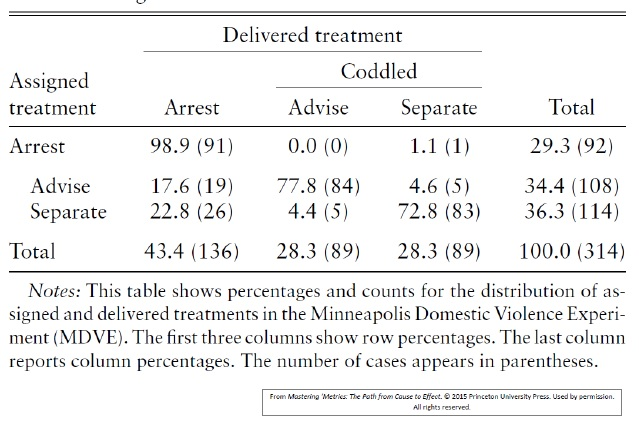
\includegraphics[width=6.5cm,height=6.5cm,keepaspectratio]{Table 3.3} 

\column{.45\textwidth}
\begin{itemize}
	\item in practice the officer's reaction often deviated
	\item treatment delivered was not random
	\item a case assigned to be coddled was coddled with a probability of .797
	\item a case assigned to be arrested was coddled with a probability of .011
\end{itemize}

\end{columns}

\end{frame}
%------------------------------------------------

\begin{frame}
\frametitle{The Minneapolis Domestic Violence Experiment (MDVE)}
\begin{itemize}
\item naive analysis of the MDVE based on treatment delivered is misleading
\item comparison of those who were and were not coddled is contaminated by selection bias
\item we need an IV analysis in order to capture the effect of treatment on the treated!
\end{itemize}

\end{frame}
%------------------------------------------------

\begin{frame}
\frametitle{IV in the MDVE}

\begin{itemize}
	\item First Stage: difference between the probability of being coddled when assigned to be coddled and the probability of being coddled when assigned to be arrested 
	\item We use $Z_i$ indicating assignment to coddling and $D_i$ indicating incidents where coddling was delivered:
	$$E[D_i|Z_i=1]-E[D_i|Z_i=0] = .797 -.011 = .786 $$
	\item we now calculate the effect of random assignment to coddling on the outcome variable $Y_i$:
	$$E[Y_i|Z_i=1]-E[Y_i|Z_i=0] = .211 - .097 = .114 $$
	\item overall recidivism rate was 18 \%, so the difference of 11 \% is substantial
\end{itemize}
\end{frame}
%------------------------------------------------
\begin{frame}
\frametitle{IV in the MDVE}
\begin{itemize}
\item in experiments where treatment assigned differs from treatment delivered, we need to calculate the effects of random assignment
\item these effects are called intention-to-treat (ITT)
\item an ITT analysis captures the causal effect of being assigned to treatment
\item ITT effect does not take the noncompliance of those assigned to be coddled and turning out to be arrested into account
\item ITT is too small!
\item therefore, we have to divide the ITT effects by the difference in compliance rates between treatment and control groups in order to capture the causal effect of coddling on compliers who were coddled as a result of the experiment
\end{itemize}

\end{frame}
%------------------------------------------------
\begin{frame}
\frametitle{IV in the MDVE}
\begin{itemize}
\item ITT is a reduced form for a randomly assigned instrument (here assignment to being coddled)
\item the IV causal chain begins with random assignment to treatment, then goes through treatment delivered and in the end affects outcomes
\item the LATE from the MDVE is $\frac{.114}{.786}=.145$, showing a large coddling effect even in comparison with the corresponding ITT estimates
\item exclusion restriction: requires that randomly assigned form color affect recidivism only through the decision to arrest or coddle
\end{itemize}

\end{frame}
%------------------------------------------------
\begin{frame}
\frametitle{IV in the MDVE}
\begin{itemize}
\item If we had ignored the nonrandom nature, we would have calculated a smaller effect:
$$E[Y_i|D_i=1]-E[Y_i|D_i=0] = .216 - .129 = .087$$
\item as seen in Chapter 1, comparison of treated and untreated without random assignment equals the causal effect plus selection bias
\item in the MDVE, batteres who were arrested although being assigned to coddled were especially violent
\item batteres who were coddled were less likely to abuse again in any case
\item selection bias does matter here!
\item IV analysis eliminates selection bias, capturing the average causal effect on compliers

\end{itemize}

\end{frame}
%------------------------------------------------
\begin{frame}
\frametitle{MDVE Conclusions}
\begin{itemize}
\item always-takers would be suspected batteres who were coddled without being assigned to coddled
\item In the MDVE we have practilly no always-takers 
\item therefore, all of the treated are compliers and LATE is TOT
\item when applying this property of the MDVE, we see that LATE is the average causal effect of coddling on the coddled
\item when some of those randomly assigned to treatment go untreated but no one assigned to control group gets treated, IV methods using random intention to treat as an instrument for treatment delivered captures TOT

\end{itemize}

\end{frame}

%------------------------------------------------


%Chapter 3.3:ab hier neu eingefugt am 15.05.
%---------------------------------------------------

\section{Family Size and Living Standards}
\begin{frame}
\frametitle{The Population Bomb}
\begin{itemize}
	\item We want to take a look at the relationship between family size and living standards
	\item We might indeed expect increases in family size to be associated with increased poverty and reduced education
		\begin{itemize}
			\item [\rightarrow] more mouths to feed means less for each
		\end{itemize}
	\item Gary Becker: introduced the notion of a quantity-quality tradeoff, the idea that reductions in family size increase parental investment in children, e.g. invest more in their schooling
\item Is there a causal connection between family size and children’s education?
\item Identification Problem: inability in principle to identify a best estimate of the value(s) of one or more parameters in a regression. 
\end{itemize}

\end{frame}


%------------------------------------------------

\begin{frame}
\frametitle{Random Assignment}
\begin{itemize}
	\item Marked differences in observable characteristics across families of different sizes raise the red flag of
selection bias.
	\item women with different numbers of children are observably different
	\item But: we must acknowledge the possibility of important unobserved differences associated with family size as well
	\item Solution: random assignment: 
	\begin{itemize}
		\item[i.] Draw a sample of families with one child.
		\item[ii.] In some of these households, randomly distribute an additional child.
		\item[iii.] Wait 20 years and collect data on the educational attainment of firstborns who did and did not get an extra sibling.
	\end{itemize}
	\item Unlikely experiment to happen, we need another way.
\end{itemize}

\end{frame}

%--------------------------------------------

\begin{frame}
\frametitle{Differences in Family Size}

\begin{itemize}
	\item Random variation in family size by sometimes having more than one child in the form of twins
	\item Large sample from Israel exploits this.
	\item Good case study: diverse population, including many people who were born in developing countries and into large families.
	\item Consider a family in which the second birth is a singleton. On average, such families include 3.6 children. A second twin birth increases average family size by .32,
	\item The .32 twins differential in family size reflects a difference in probabilities: the likelihood of having a third child increases from about .7 with a singleton second birth to a certainty
\end{itemize}

\end{frame}

%--------------------------------------------

\begin{frame}
\frametitle{Using of IV Estimates}
\begin{itemize}
	\item We use twin births as an instrument for family size.
	\item The comparison of schooling between firstborns with twin and singleton siblings constitutes the reduced form for an IV estimate.
	\item IV estimates are constructed from the ratio of reduced-form to first-stage estimates
	\item Here: The fact that the twins reduced form and associated IV estimates are close to zero weighs against the view that a larger family of origin reduces children’s schooling.
	\item But: potentially omitted variables due to non random assignment.
\end{itemize}

\end{frame}

%--------------------------------------------

\begin{frame}
\frametitle{Another Option}
\begin{itemize}
	\item Many parents hope for a diversified sibling-sex portfolio: Families whose first two children are both boys or both girls are more likely to have a third.
	\item Sex of a newborn is randomly assigned.
	\item Parental preferences for mixed sibling-sex composition generate an instrument.
	\item First-born Israeli adults who have a second-born sibling of the opposite sex grew up in households with about 3.60 children.
	\item But firstborns whose second-born sibling is of the same sex were raised in families with 3.68 children. 	
	\item The same-sex first stage for Israeli firstborns is about .08.
\end{itemize}

\end{frame}

%--------------------------------------------

\begin{frame}
\frametitle{The IV Variable}
	\item Instrumental variable is a dummy variable that equals 1 for families whose first two children are both male or both female and equals 0 for families with one boy and one girl.
	\item But: the educational attainment of first-born Israeli adults is unaffected by their siblings’ sex composition.
	\item IV has an effect on the treatment (family size) and should only effect the outcome (Education) through the treatment (family size) $\rightarrow Exclusion~restriction.$
	\item But: Might the sex-mix of the first two children affect childrens educational outcomes for other reasons?
	\item Maybe same sex childs have the benefit of using the same clothing etc. so the family is a bit richer which increases parental investment in their children’s schooling.
\end{frame}

%--------------------------------------------
\begin{frame}
\frametitle{Test exclusion restriction}
\begin{itemize}
	\item Test exclusion restriction: 
	\item Because the fertility of always-takers and never-takers is unchanged by sibling sex composition, any relationship between sex-mix instruments and outcomes in samples with few compliers may signal violations of the underlying exclusion restriction.
	\item Help with using LATE: The ratio of reduced-form to first-stage parameters, that is:
	$$\lambda = \frac{\rho}{\phi} $$

\end{itemize}
\end{frame}

%------------------------------------------------
\begin{frame}
\frametitle{Recap: First Stage and Reduced Form}

\begin{itemize}
	\item When the first stage, $\phi$, is zero, the reduced form should be zero as well.
	\item[\rightarrow] Where the effect of the instrument on the treatment variable is zero, the reduced form should be zero.
	\item Reduced-form estimate with no evidence of a corresponding first stage is cause for worry, because this suggests some channel other than the treatment variable (in this case, family size) links
instruments with outcomes.
	\item[\rightarrow] Would mean that the instrument does not effect the treatment variables, but the outcome, so it would violate the exclusion restriction.
	\item Also the instrument should not correlate with the error term.
\end{itemize}

\end{frame}

%--------------------------------------------

\begin{frame}
\frametitle{2SLS Regression}
\begin{itemize}
	\item Assume twins and sex-mix instruments both satisfy the required assumptions and capture similar average causal effects.
	\begin{itemize}
		\item[\rightarrow] Combining the two IV estimates, they increase statistical precision.
	\end{itemize}
	\item Potential bias: We must control for confounding factors
	\item Solution: Two-stage least squares (2SLS) generalizes IV in two ways:
	\begin{itemize}
		\item[i.] 2SLS estimates use multiple instruments efficiently.
		\item[ii.] 2SLS estimates control for covariates, thereby mitigating OVB from imperfect instruments.
	\end{itemize}
\end{itemize}

\end{frame}

%--------------------------------------------

\begin{frame}
\frametitle{Using regular Regression}

\begin{itemize}
	\item Reduced Form: dummy variable for multiple second births denoted by $Z_i$, the reduced-form
effect can be written as the coefficient $\rho$ in the regression equation: 
$$Y_i=\alpha_0 + \rho Z_i + \epsilon_{0i}$$
\item First Stage: Likewise, the first-stage effect of $Z_i$ is the coefficient $\phi$ in the first-stage equation: 
$$D_i=\alpha_1 + \phi Z_i + \epsilon_{1i}$$
\item LATE is the ratio of the slope coefficients: 
$$\lambda = \frac{\rho}{\phi}$$

\end{itemize}

\end{frame}

%--------------------------------------------

\begin{frame}
\frametitle{Using 2SLS Regression}

\begin{itemize}
	\item The 2SLS procedure offers an alternative way of computing $\lambda = \frac{\rho}{\phi}$
	\item In the 2SLS first stage, we estimate $D_i=\alpha_1 + \phi Z_i + \epsilon_{1i}$ and save the fitted values. 
	\item These “first-stage fits” are defined as: 
	$$\hat{D_i}=\alpha_1 + \phi Z_i $$
	\item The 2SLS second stage regresses Yi on Di, as in: 
	$$Y_i=\alpha_2+\lambda_{2SLS}\hat{D_i}+\epsilon_{2i}$$
	\item The value of $\lambda_{2SLS}$ generated by this second step is identical to the ratio of reduced form to first-stage regression coefficients, $\frac{\rho}{\phi}$.

\end{itemize}

\end{frame}

%--------------------------------------------
\begin{frame}
\frametitle{Remember: Fitted Values}
\begin{columns}
\column{.5\textwidth}
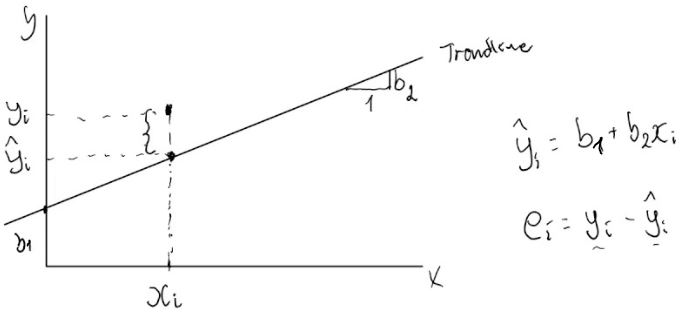
\includegraphics[width=6.5cm,height=6.5cm,keepaspectratio]{Fitted Values} 

\column{.45\textwidth}
\begin{itemize}
	\item Fitted value $\hat{y_i}$ is the prediction of the mean response value when you input the values of the predictors into the model.
	\item Also called predicted values.
	\item The difference between fitted values and real values is my residuum.
\end{itemize}

\end{columns}
\end{frame}

%--------------------------------------------
\begin{frame}
\frametitle{Using 2SLS Regression}

\begin{itemize}
	\item Adding maternal age, denoted $A_i$, the reduced form and first stage look like (influence of twins on Education and family size):
	\begin{flalign*}
			Reduced~ Form:Y_i=\alpha_0 + \rho Z_i + \gamma_0 A_i + \epsilon_{0i}\\
			First~ Stage:D_i=\alpha_1 + \phi Z_i +\gamma_1 A_i + \epsilon_{1i}
			\end{flalign*}
	\item Again, we need the first Stage fitted Values: $\hat{D_i}=\alpha_1 + \phi Z_i+ \gamma_1 A_i$
	\item 2SLS estimates are again constructed by regressing $Y_i$ on both $\hat{D_i}$ and $A_i$. Hence, the 2SLS second-stage equation is (Influence of Family Size on Education):
$$Y_i=\alpha_2+\lambda_{2SLS}\hat{D_i}+\gamma_2 A_i +\epsilon_{2i}$$

\end{itemize}

\end{frame}

%--------------------------------------------

\begin{frame}
\frametitle{Benefits of 2SLS}

\begin{itemize}
	\item Benefit of this model: The 2SLS setup allows as many control variables as you like, provided they appear in both the first and second stages.
	\item Econometrics software packages compute 2SLS estimates directly, reducing the scope for mistakes
	\item Another benefit: Multiple instruments useable: e.g. dummy for same-sex siblings $(W_i)$, need to add a dummy, $B_i$, indicating first-born boys.
	\item But: 2SLS is nothing else then 2 OLS Regressions: A first and a second stage.
	\item Remember: OLS: statistical algorithm to minimize the sum of least squares.
\end{itemize}
\end{frame}
%--------------------------------------------

\begin{frame}
\frametitle{Using 2SLS Regression}
\begin{itemize}
	\item With two instruments, $W_i$ and $Z_i$, and the extra control variable, $B_i$, the 2SLS first stage becomes:
$$D_i=\alpha_1 + \phi_t Z_i +\phi_s W_i +\gamma_1 A_i + \delta_1 B_i + \epsilon_{1i}$$
	\item reduced form: 
$$Y_i=\alpha_0 + \rho_t Z_i +\rho_s W_i + \gamma_0 A_i +\delta_0 B_i +  \epsilon_{0i}$$
	\item Second-stage estimates with two instruments and two covariates are generated by the regression equation: 
$$Y_i=\alpha_2+\lambda_{2SLS}\hat{D_i}+\gamma_2 A_i +\delta_2 B_i + \epsilon_{2i} $$
	\item This produces a weighted average of the estimates we get using the instruments $Z_i$ and $W_i$ one at a time, while controlling for covariates $A_i$ and $B_i$.

\end{itemize}

\end{frame}
%----------------------------------------------------------------------------------------
\begin{frame}
\frametitle{Quality-Quantity Trade Off}

\begin{columns}
\column{.5\textwidth}
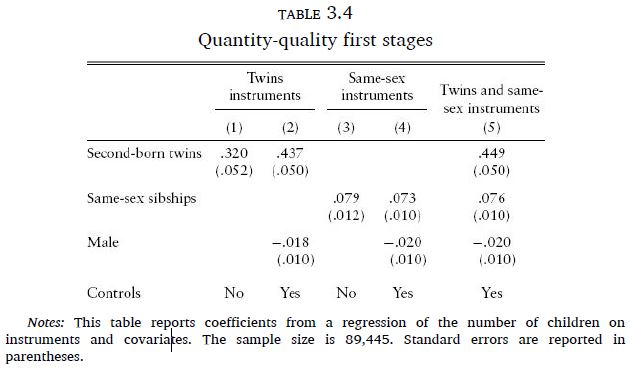
\includegraphics[width=6.5cm,height=6.5cm,keepaspectratio]{Table 3.4} 

\column{.45\textwidth}
\begin{itemize}
	\item Second born twins increase the number of children to 0.32 more
	\item First-born Israeli adults whose second-born siblings were twin were raised in families with about .44 more children than those raised in families where the second birth was a singleton.

\end{itemize}

\end{columns}
\end{frame}
%----------------------------------------------------------------------------------------

\begin{frame}
\frametitle{OLS and 2SLS Estimates}

\begin{columns}
\column{.5\textwidth}
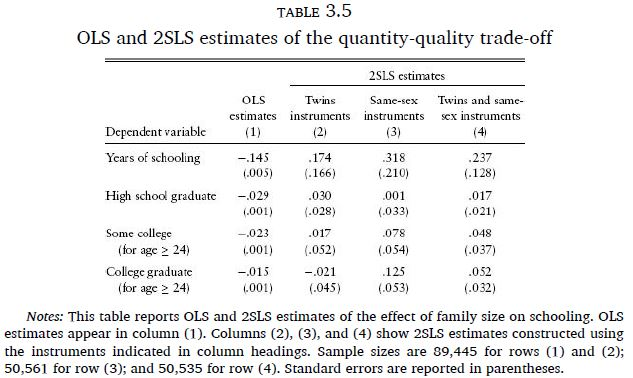
\includegraphics[width=6.5cm,height=6.5cm,keepaspectratio]{Table 3.5} 

\column{.45\textwidth}
\begin{itemize}
	\item OLS shows a strong negative relation between family size and education outcomes.
	\item 2SLS estimates in column (3) show uniformly positive effects of family size on education.
\end{itemize}

\end{columns}
\end{frame}
%----------------------------------------------------------------------------------------
\begin{frame}
\frametitle{Summary}

\begin{itemize}
	\item The pooled second-stage estimates are not very different from those generated using the instruments one at a time, but the standard errors are appreciably smaller.
\begin{itemize}
	\item[\rightarrow] Can increase precision by pooling multiple instruments
\end{itemize}
\item Findings here suggest that the strong negative association between family size and schooling is driven in large part and perhaps entirely by selection bias.
\end{itemize}
\end{frame}

%----------------------------------------------------------------------------------------
\begin{frame}
\frametitle{In a nutshell}

\begin{itemize}
	\item Foundation has three layers: 
	\begin{itemize}
		\item[i] the first-stage requires instruments that affect the causal channel of interest; 
		\item[ii] the independence assumption requires instruments to be as good as randomly assigned; 
		\item[iii] the exclusion restriction asserts that a single causal channel connects instruments with outcomes.
	\end{itemize}
	\item Check those assumptions:
\begin{itemize}
	\item[i] First stage: By looking for a strong relationship between instruments and the proposed causal channel;
	\item[ii] Independence assumption: By checking covariate balance with the instrument switched off and on, as in a randomized trial.
	\item[iii] Exclusion restriction: Hard to check, in sample with small first stage, Exclusion implies such samples should generate small reduced-form estimates
\end{itemize}


\end{itemize}
\end{frame}


%--------------------------------------------
\section{Appendix}
\begin{frame}
\frametitle{Appendix}

\begin{itemize}
	\item IV setup with one instrument and no covariates. 
	\item The first stage links instrument and treatment: 
	$$D_i=\alpha_1 + \phi Z_i + \epsilon_{1i}$$
	\item The reduced form links instrument and outcomes: 
	$$Y_i=\alpha_0 + \rho Z_i + \gamma_0 A_i + \epsilon_{0i}$$
	\item The 2SLS second stage is the regression of outcomes on first-stage fitted values:
	$$Y_i=\alpha_2+\lambda_{2SLS}\hat{D_i}+\gamma_2 A_i +\epsilon_{2i}$$
	\item With ratio of covariances $\rho~ and~ \phi, ~\lambda$ is called the IV formula:
	$$\lambda = \frac{\rho}{\phi}$$
	\item If you have Covariates, e.g. $A_i$, include them in the model, no change to the IV formula (or 2sls Formula)
\end{itemize}
\end{frame}

%----------------------------------------------------------------------------------------
\begin{frame}
\frametitle{2SLS Standard Errors}

\begin{itemize}
	\item First the 2SLS residual is constructed using: 
	$$\eta_i=Y_i-\alpha_2-\lambda_{2SLS} D_i - \gamma_2 A_i.$$
	\item $\sigma{\eta}$ is the standard deviation of $\eta_i$
	\item The standard error for lambda is then given by: 
	$$SE(\hat{\lambda}_{2SLS})=\frac{\sigma_{\eta}}{\sqrt{n}}\times \frac{1}{\sigma_{\hat{D}}}$$
	\item 2SLS combines multiple instruments in an effort to generate precise estimates of a single causal effect.
	\item Problem: 2SLS estimates with many weak instruments can be misleading.
	\item How do I know that an instrument is weak: one that isn’t highly correlated with the regressor being instrumented, so the first-stage coefficient associated with this instrument is small or imprecisely estimated. Then 2SLS is close to OLS.
\end{itemize}
\end{frame}

%----------------------------------------------------------------------------------------
\begin{frame}
\frametitle{2SLS Bias}

\begin{itemize}
	\item Finite sample bias: 2SLS estimates in a many weak IV scenario tell you little about the causal relationship of interest.
	\item Solution: An alternative to 2SLS, called the limited information maximum likelihood estimator (LIML for short) is less affected by finite sample bias. You’d like LIML estimates and 2SLS estimates to be close to one another, since the former are unlikely to be biased even with many weak instruments.
	\item But: finite sample bias does not occur, when you only use one instrument.
	\item Reduced-form estimates that are small and not significantly different from zero provide a strong and unbiased hint that the causal relationship of interest is weak or nonexistent.
\end{itemize}
\end{frame}

%----------------------------------------------------------------------------------------
\begin{frame}
\Huge{\centerline{Thank you very much for listening}}
\end{frame}

%----------------------------------------------------------------------------------------

\end{document} 